\documentclass{report}

\setcounter{tocdepth}{3} % put subsubsections in TOC
\usepackage{url}
\usepackage[utf8]{inputenc}
\usepackage[toc,page]{appendix}
\linespread{1.5}

%%% For syntax highlight in Sphinx generated listing codes
%% graphicx and hyperref must not be reimported
\usepackage{sphinx}

\makeatletter
\def\PYG@reset{\let\PYG@it=\relax \let\PYG@bf=\relax%
    \let\PYG@ul=\relax \let\PYG@tc=\relax%
    \let\PYG@bc=\relax \let\PYG@ff=\relax}
\def\PYG@tok#1{\csname PYG@tok@#1\endcsname}
\def\PYG@toks#1+{\ifx\relax#1\empty\else%
    \PYG@tok{#1}\expandafter\PYG@toks\fi}
\def\PYG@do#1{\PYG@bc{\PYG@tc{\PYG@ul{%
    \PYG@it{\PYG@bf{\PYG@ff{#1}}}}}}}
\def\PYG#1#2{\PYG@reset\PYG@toks#1+\relax+\PYG@do{#2}}

\expandafter\def\csname PYG@tok@gd\endcsname{\def\PYG@tc##1{\textcolor[rgb]{0.63,0.00,0.00}{##1}}}
\expandafter\def\csname PYG@tok@gu\endcsname{\let\PYG@bf=\textbf\def\PYG@tc##1{\textcolor[rgb]{0.50,0.00,0.50}{##1}}}
\expandafter\def\csname PYG@tok@gt\endcsname{\def\PYG@tc##1{\textcolor[rgb]{0.00,0.27,0.87}{##1}}}
\expandafter\def\csname PYG@tok@gs\endcsname{\let\PYG@bf=\textbf}
\expandafter\def\csname PYG@tok@gr\endcsname{\def\PYG@tc##1{\textcolor[rgb]{1.00,0.00,0.00}{##1}}}
\expandafter\def\csname PYG@tok@cm\endcsname{\let\PYG@it=\textit\def\PYG@tc##1{\textcolor[rgb]{0.25,0.50,0.56}{##1}}}
\expandafter\def\csname PYG@tok@vg\endcsname{\def\PYG@tc##1{\textcolor[rgb]{0.73,0.38,0.84}{##1}}}
\expandafter\def\csname PYG@tok@m\endcsname{\def\PYG@tc##1{\textcolor[rgb]{0.13,0.50,0.31}{##1}}}
\expandafter\def\csname PYG@tok@mh\endcsname{\def\PYG@tc##1{\textcolor[rgb]{0.13,0.50,0.31}{##1}}}
\expandafter\def\csname PYG@tok@cs\endcsname{\def\PYG@tc##1{\textcolor[rgb]{0.25,0.50,0.56}{##1}}\def\PYG@bc##1{\setlength{\fboxsep}{0pt}\colorbox[rgb]{1.00,0.94,0.94}{\strut ##1}}}
\expandafter\def\csname PYG@tok@ge\endcsname{\let\PYG@it=\textit}
\expandafter\def\csname PYG@tok@vc\endcsname{\def\PYG@tc##1{\textcolor[rgb]{0.73,0.38,0.84}{##1}}}
\expandafter\def\csname PYG@tok@il\endcsname{\def\PYG@tc##1{\textcolor[rgb]{0.13,0.50,0.31}{##1}}}
\expandafter\def\csname PYG@tok@go\endcsname{\def\PYG@tc##1{\textcolor[rgb]{0.20,0.20,0.20}{##1}}}
\expandafter\def\csname PYG@tok@cp\endcsname{\def\PYG@tc##1{\textcolor[rgb]{0.00,0.44,0.13}{##1}}}
\expandafter\def\csname PYG@tok@gi\endcsname{\def\PYG@tc##1{\textcolor[rgb]{0.00,0.63,0.00}{##1}}}
\expandafter\def\csname PYG@tok@gh\endcsname{\let\PYG@bf=\textbf\def\PYG@tc##1{\textcolor[rgb]{0.00,0.00,0.50}{##1}}}
\expandafter\def\csname PYG@tok@ni\endcsname{\let\PYG@bf=\textbf\def\PYG@tc##1{\textcolor[rgb]{0.84,0.33,0.22}{##1}}}
\expandafter\def\csname PYG@tok@nl\endcsname{\let\PYG@bf=\textbf\def\PYG@tc##1{\textcolor[rgb]{0.00,0.13,0.44}{##1}}}
\expandafter\def\csname PYG@tok@nn\endcsname{\let\PYG@bf=\textbf\def\PYG@tc##1{\textcolor[rgb]{0.05,0.52,0.71}{##1}}}
\expandafter\def\csname PYG@tok@no\endcsname{\def\PYG@tc##1{\textcolor[rgb]{0.38,0.68,0.84}{##1}}}
\expandafter\def\csname PYG@tok@na\endcsname{\def\PYG@tc##1{\textcolor[rgb]{0.25,0.44,0.63}{##1}}}
\expandafter\def\csname PYG@tok@nb\endcsname{\def\PYG@tc##1{\textcolor[rgb]{0.00,0.44,0.13}{##1}}}
\expandafter\def\csname PYG@tok@nc\endcsname{\let\PYG@bf=\textbf\def\PYG@tc##1{\textcolor[rgb]{0.05,0.52,0.71}{##1}}}
\expandafter\def\csname PYG@tok@nd\endcsname{\let\PYG@bf=\textbf\def\PYG@tc##1{\textcolor[rgb]{0.33,0.33,0.33}{##1}}}
\expandafter\def\csname PYG@tok@ne\endcsname{\def\PYG@tc##1{\textcolor[rgb]{0.00,0.44,0.13}{##1}}}
\expandafter\def\csname PYG@tok@nf\endcsname{\def\PYG@tc##1{\textcolor[rgb]{0.02,0.16,0.49}{##1}}}
\expandafter\def\csname PYG@tok@si\endcsname{\let\PYG@it=\textit\def\PYG@tc##1{\textcolor[rgb]{0.44,0.63,0.82}{##1}}}
\expandafter\def\csname PYG@tok@s2\endcsname{\def\PYG@tc##1{\textcolor[rgb]{0.25,0.44,0.63}{##1}}}
\expandafter\def\csname PYG@tok@vi\endcsname{\def\PYG@tc##1{\textcolor[rgb]{0.73,0.38,0.84}{##1}}}
\expandafter\def\csname PYG@tok@nt\endcsname{\let\PYG@bf=\textbf\def\PYG@tc##1{\textcolor[rgb]{0.02,0.16,0.45}{##1}}}
\expandafter\def\csname PYG@tok@nv\endcsname{\def\PYG@tc##1{\textcolor[rgb]{0.73,0.38,0.84}{##1}}}
\expandafter\def\csname PYG@tok@s1\endcsname{\def\PYG@tc##1{\textcolor[rgb]{0.25,0.44,0.63}{##1}}}
\expandafter\def\csname PYG@tok@gp\endcsname{\let\PYG@bf=\textbf\def\PYG@tc##1{\textcolor[rgb]{0.78,0.36,0.04}{##1}}}
\expandafter\def\csname PYG@tok@sh\endcsname{\def\PYG@tc##1{\textcolor[rgb]{0.25,0.44,0.63}{##1}}}
\expandafter\def\csname PYG@tok@ow\endcsname{\let\PYG@bf=\textbf\def\PYG@tc##1{\textcolor[rgb]{0.00,0.44,0.13}{##1}}}
\expandafter\def\csname PYG@tok@sx\endcsname{\def\PYG@tc##1{\textcolor[rgb]{0.78,0.36,0.04}{##1}}}
\expandafter\def\csname PYG@tok@bp\endcsname{\def\PYG@tc##1{\textcolor[rgb]{0.00,0.44,0.13}{##1}}}
\expandafter\def\csname PYG@tok@c1\endcsname{\let\PYG@it=\textit\def\PYG@tc##1{\textcolor[rgb]{0.25,0.50,0.56}{##1}}}
\expandafter\def\csname PYG@tok@kc\endcsname{\let\PYG@bf=\textbf\def\PYG@tc##1{\textcolor[rgb]{0.00,0.44,0.13}{##1}}}
\expandafter\def\csname PYG@tok@c\endcsname{\let\PYG@it=\textit\def\PYG@tc##1{\textcolor[rgb]{0.25,0.50,0.56}{##1}}}
\expandafter\def\csname PYG@tok@mf\endcsname{\def\PYG@tc##1{\textcolor[rgb]{0.13,0.50,0.31}{##1}}}
\expandafter\def\csname PYG@tok@err\endcsname{\def\PYG@bc##1{\setlength{\fboxsep}{0pt}\fcolorbox[rgb]{1.00,0.00,0.00}{1,1,1}{\strut ##1}}}
\expandafter\def\csname PYG@tok@kd\endcsname{\let\PYG@bf=\textbf\def\PYG@tc##1{\textcolor[rgb]{0.00,0.44,0.13}{##1}}}
\expandafter\def\csname PYG@tok@ss\endcsname{\def\PYG@tc##1{\textcolor[rgb]{0.32,0.47,0.09}{##1}}}
\expandafter\def\csname PYG@tok@sr\endcsname{\def\PYG@tc##1{\textcolor[rgb]{0.14,0.33,0.53}{##1}}}
\expandafter\def\csname PYG@tok@mo\endcsname{\def\PYG@tc##1{\textcolor[rgb]{0.13,0.50,0.31}{##1}}}
\expandafter\def\csname PYG@tok@mi\endcsname{\def\PYG@tc##1{\textcolor[rgb]{0.13,0.50,0.31}{##1}}}
\expandafter\def\csname PYG@tok@kn\endcsname{\let\PYG@bf=\textbf\def\PYG@tc##1{\textcolor[rgb]{0.00,0.44,0.13}{##1}}}
\expandafter\def\csname PYG@tok@o\endcsname{\def\PYG@tc##1{\textcolor[rgb]{0.40,0.40,0.40}{##1}}}
\expandafter\def\csname PYG@tok@kr\endcsname{\let\PYG@bf=\textbf\def\PYG@tc##1{\textcolor[rgb]{0.00,0.44,0.13}{##1}}}
\expandafter\def\csname PYG@tok@s\endcsname{\def\PYG@tc##1{\textcolor[rgb]{0.25,0.44,0.63}{##1}}}
\expandafter\def\csname PYG@tok@kp\endcsname{\def\PYG@tc##1{\textcolor[rgb]{0.00,0.44,0.13}{##1}}}
\expandafter\def\csname PYG@tok@w\endcsname{\def\PYG@tc##1{\textcolor[rgb]{0.73,0.73,0.73}{##1}}}
\expandafter\def\csname PYG@tok@kt\endcsname{\def\PYG@tc##1{\textcolor[rgb]{0.56,0.13,0.00}{##1}}}
\expandafter\def\csname PYG@tok@sc\endcsname{\def\PYG@tc##1{\textcolor[rgb]{0.25,0.44,0.63}{##1}}}
\expandafter\def\csname PYG@tok@sb\endcsname{\def\PYG@tc##1{\textcolor[rgb]{0.25,0.44,0.63}{##1}}}
\expandafter\def\csname PYG@tok@k\endcsname{\let\PYG@bf=\textbf\def\PYG@tc##1{\textcolor[rgb]{0.00,0.44,0.13}{##1}}}
\expandafter\def\csname PYG@tok@se\endcsname{\let\PYG@bf=\textbf\def\PYG@tc##1{\textcolor[rgb]{0.25,0.44,0.63}{##1}}}
\expandafter\def\csname PYG@tok@sd\endcsname{\let\PYG@it=\textit\def\PYG@tc##1{\textcolor[rgb]{0.25,0.44,0.63}{##1}}}

\def\PYGZbs{\char`\\}
\def\PYGZus{\char`\_}
\def\PYGZob{\char`\{}
\def\PYGZcb{\char`\}}
\def\PYGZca{\char`\^}
\def\PYGZam{\char`\&}
\def\PYGZlt{\char`\<}
\def\PYGZgt{\char`\>}
\def\PYGZsh{\char`\#}
\def\PYGZpc{\char`\%}
\def\PYGZdl{\char`\$}
\def\PYGZhy{\char`\-}
\def\PYGZsq{\char`\'}
\def\PYGZdq{\char`\"}
\def\PYGZti{\char`\~}
% for compatibility with earlier versions
\def\PYGZat{@}
\def\PYGZlb{[}
\def\PYGZrb{]}
\makeatother

%%% For syntax highlight in Sphinx generated listing codes

\begin{document}

\title{Diderot - A Test Driven Development Tool for developing RDF/OWL ontologies}
\author{
Ícaro Medeiros\\
Registration (Matrícula) 1212403
\\ \\ \\ \\ \\ \\ \\ \\
Pontifical Catholic University of Rio de Janeiro \\
Doctorate in Computer Science \\
INF 2102 - Programming Final Project (Projeto final de Programação) \\
Coordinator: Prof. Arndt Von Staa \\
Advisor: Prof. Daniel Schwabe
}

\maketitle
\tableofcontents

\chapter{Introduction}

Test Driven Development (TDD) techniques have been successfully used in software engineering \cite{beck03}, providing an iterative, agile and incremental way of developing code.
In this approach, programmers start by writing tests for their code, then programming the code so the tests do not fail.
Then the code can be enhanced and checked against tests again, completing a desirable test-write-refactor cycle.

TDD is a safe methodology to develop programs, where we can be sure that changes do not introduce bugs or unexpected behavior by running our automated tests for our code.
Moreover, by doing tests first, we can check our architecture decisions simply by being clients of our own code in our tests. And finally the tests can also be seen as a documentation about the code.

Almost all modern programming languages have unit test frameworks that enable to run automated tests for your code and engage into a TDD process for software, such as the xUnit framework \cite{beck03} and its implementations (JUnit, Python unit testing framework, etc).

In a TDD approach you can start with simple software units, in a bottom-up way,
rather than over modeling all your system in advance, the so called Big Design Up Front (BDUF).
This leads to code that can rapidly be released, in short cycles, enabling early releases of
shipable software for the clients to validate and provide feedback, a premise in Agile
Software Process Methodologies \cite{beck01, beck04, martin03}.

Ontology engineering could benefit from a TDD process like this, using small iterations
to ensure a good quality ontology, consistent, well tested and ready for evolution.

\section{Test Driven Development for Ontologies}

During the ontology development authors might not be aware what kinds of inferences their ontologies are
providing, for example, if a new rule introduced unexpected inference. Checking the ontology for
self-consistency is also a demanding task.

As stated in \cite{vrandevcic06}, the idea of design by contract, well known in Software Engineering can
be used to Ontology Engineering as follows: we could declare what statements should and
should not derive from an ontology being developed. Thus we can be sure if expected inferences are
derived and be aware of unexpected inferred conclusions.

Moreover, competency questions, as defined by some methodologies for Ontology Engineering like Methontology \cite{lopez99},
describe what kind of knowledge the resulting ontology is supposed to answer. These questions can always be formalized in
a query language (like SPARQL). By formalizing the queries and the expected answers, a system can automatically checks if
the ontology meets the requirements stated in the competency questions.

To answer these needs in this report a novel Test Driven Development tool for building RDF/OWL ontologies is proposed, called
Diderot. This report is organized as follows: the Chapter \ref{system} describes the requirements, use cases, architecture and
how Diderot was built. In Chapter \ref{manual} it is described how to use Diderot in all its use cases, including installation and
documentation. Finally, in Chapter \ref{conclusion} we present concluding remarks and future goals for the project.

\chapter{System Description}
\label{system}

This chapter will describe the goals defined for Diderot, a tool for Test Driven Development for building RDF/OWL ontologies
and how the system was built, including use cases, architecture and the engineering process.

\section{Goals}
\label{goals}

The main goals of Diderot is to provide a simple interface to test small portions of ontologies regarding:

\begin{itemize}
    \item Expected inferences. The system must check if expected inferences are satisfied by the ontology
        given as input.
    \item Check for lack of unexpected inferences. The system must guarantee that no unexpected inferences are
        derived from the target ontology.
    \item Answering competency questions. The system must check if answers to competency questions are
        the same as users expect, given the target ontologies and the knowledge base which uses the ontology.
\end{itemize}

\section{Requirements}
\label{requirements}

The requirements of Diderot follows:
\begin{itemize}
    \item To provide facilities for testing ontologies regarding the goals mentioned in Section \ref{goals}: cheking
        expected and lack of unexpected inferences, self consistency and proper competency questions answering.
    \item The input to the system should be made in many formats possible, such as Turtle format for RDF serialization,
        as a simple way of writting RDF. The input might be a string representing RDF in Turtle format, a file or a
        URI that contains a RDF ontology. Also, it is desirable to provide a SPARQL interface to writting competency questions.
    \item To provide a simple Domain Specific Language for writting tests for ontologies. The API of the tool must be simple
        to use and extend to cover different test scenarios.
    \item To be written in Python. As the main language used in Globo.com having a tool written in Python is desirable.
        Moreover, the possibility to reuse tools such as RDFlib (for dealing with RDF data), the inference library FuXi
        and the Python unit testing framework lead to the requirement of using Python.
        Finally, Python is a multi-plataform language so the tool is available for all platforms that Python supports.
\end{itemize}

\subsection{Use Cases}
\label{useCases}

The use cases follow strictly the goals stated in Section \ref{goals}. A diagram summarizing the use cases is seen
in Figure \ref{figUseCase}.

\begin{figure}[!hbt]
    \centering
    \label{figUseCase}
    \caption{Use case diagram for Diderot}
    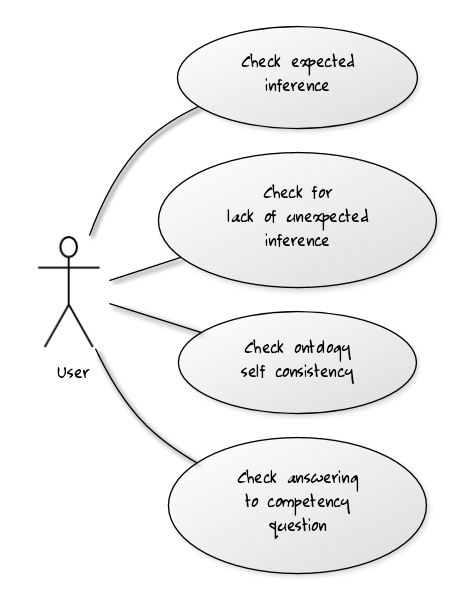
\includegraphics[scale=0.75]{fig/use_case_diagram.png}
\end{figure}

Following, the use cases will be described as user stories \cite{beck04}.

\subsubsection{Check Expected Inference}

As a ontology developer, I want to check expected inferences in ontologies so that I can develop them
in a safe way and be assure that their evolution will not break rules or invalidate previously
functional inferences.

\subsubsection{Check for lack of Unexpected Inference}

As a ontology developer, I want to check for lack of unexpected inferences so that unwanted facts
derived from the ontology do no harm ontology uses.

\subsubsection{Check Answering to Competency Question}

As a ontology developer, I want to check expected answers for competency questions that are required
so that ontology can fulfill its goal. The question can be asked as a SPARQL query.

\section{Architecture}

Diderot architecture is summarized in Figure \ref{figArchitecture}.
The \texttt{case} module is the interface with our users (programmers).
Users must extend \texttt{DiderotTestCase} (main class in \texttt{case} module) in their test cases to use Diderot.
\texttt{DiderotTestCase}, in turn, extends \texttt{TestCase} (from \texttt{unittest}, the Python unit testing framework).
In Diderot's test cases, assertions (in the \texttt{assertion} module) are used to check, for example, that expected facts can be inferred from the input ontology.

Finally, assertions use the \texttt{inference} module to trigger inferences in \texttt{FuXi}, a inference machine written in Python.
\texttt{Fuxi} uses rules that express RDF and OWL semantics to perform its inferences.

\texttt{RDFLib} and the \texttt{utils} package are used through all the code to perform utilitary functions such as parsing of ontologies written in Turtle format for RDF, checking if a \texttt{RDFLib graph} object contains a subset of triples of another object, performing SPARQL queries in memory and so on.

\begin{figure}[!hbt]
    \centering
    \label{figArchitecture}
    \caption{Diderot architecture}
    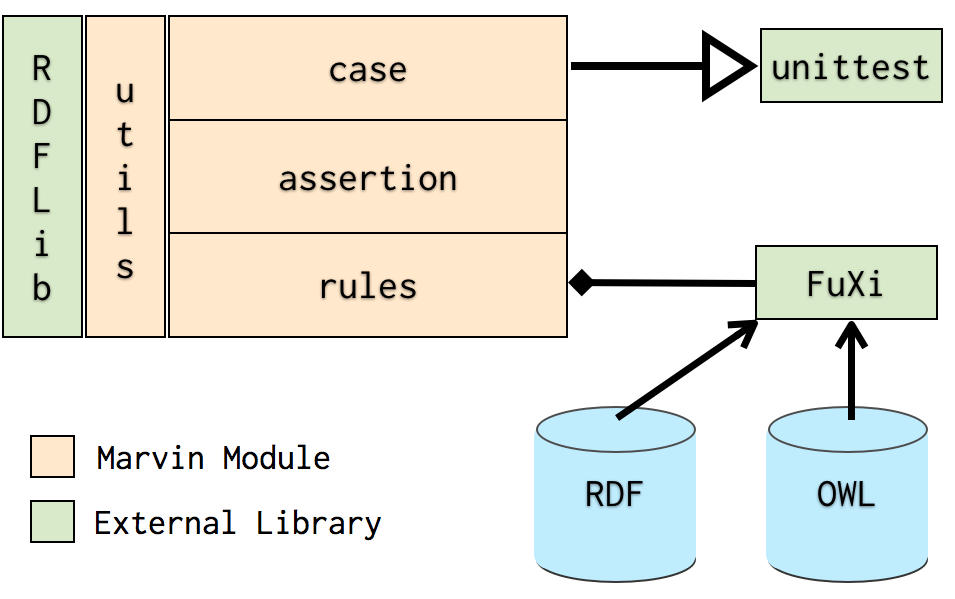
\includegraphics[scale=0.33]{fig/architecture.png}
\end{figure}

\section{Engineering Process}

During the development of Diderot, the code (and this report) was hosted in Github
\footnote{Available at \url{http://github.com/icaromedeiros/diderot}}, a social coding tool that enables free software
sharing. The Semantic Web community and all users are welcome to contribute to the project and give feedback.

Within Github users can open issues, fork the project (create your own copy) and perform pull requests (patches to the
current code to be accepted by project maintainers) and so on in order to evolve the software. As today, many
important project are hosted on Github such as linux or Rails \footnote{Available at \url{http://github.com/torvalds/linux}
and \url{http://github.com/rails/rails}}.

Git version control was used in the software development, as it is the
default system used in Github and currently the most complete and popular version control system.

We have also connected the Github project to a Continuous Integration tool\cite{beck04}. Every change pushed into Diderot's repository on github triggers automatically a run on the automated tests (fully explained in Section \ref{tests}), using the Travis CI\footnote{Available at \url{http://www.travis-ci.org/}} tool. A badge in Diderot's README file on Github presents if the build is passing or not.

As a software development methodology the Extreme Programming \cite{beck04} was chosen, with a focus on Test Driven
Development. It would be rather contradictory to build a TDD tool without using the methodology in its own development.
The tests are described next.

\subsection{Tests}
\label{tests}

In the Test Driven Development used to create Diderot different kinds of tests were used, namely:

\begin{itemize}
    \item Unit tests. Testing only small portions of code make the software APIs better, clean code safe for changes.
        It is done considering the code behind it, i.e. it is a white-box test.
    \item Functional tests. A quality assurance test that integrate multiple parts of the software and test broader
        functionalities, where nearly real data is often used.
        It is a black-box test as the internal program structure is mainly not considered.
    \item Acceptance tests. Test the software contract, i.e. if the requirements are fully satisfied. Mainly involve
        user interface tests, but as Diderot is mainly a developer tool, our acceptance tests are unit tests for ontologies
        using our tool and real examples of ontologies that test our requirements (Section \ref{requirements}).
\end{itemize}

\subsubsection{Unit Tests}

Currently, Diderot has 42 unit tests, covering 100\% of the code\footnote{Coverage percentage is extracted using coverage tool, available at \url{https://pypi.python.org/pypi/coverage}}.
Not only all the lines are tested, but all code branches (e.g. all conditional flows).

\subsubsection{Functional Tests}

Currenly, Diderot has 8 functional tests, covering broader functionalities such as asserting correct inference using different OWL capabilities.

\subsubsection{Acceptance Tests}

Acceptance tests cover all the requirements of the software to validate all the software use cases and cycles.
These tests are also used in the user manual \cite{manual} as they present real examples on how to use our tool.

\chapter{User Manual}
\label{manual}

Software documentation is rather confuse and incomplete.
A good documentation can make a real difference between low or high adopted software.
Therefore, Diderot documentation is extensive and well designed.

\section{Documentation}

The documentation is available online at \url{https://diderot.readthedocs.org}.
Using sphinx tool\footnote{Available at \url{http://sphinx-doc.org/}}, it was created documentation using
reStructuredText, a simple format to write documentation.
Sphinx compile the \texttt{.rst} files into HTML files that create a browsable and very usable documentation.
The main page of Diderot's documentation is shown in Figure \ref{figDocs}.
A use example documentation is shown in Figure \ref{figDocs2}

\begin{figure}[!hbt]
    \centering
    \label{figDocs}
    \caption{Documentation main page}
    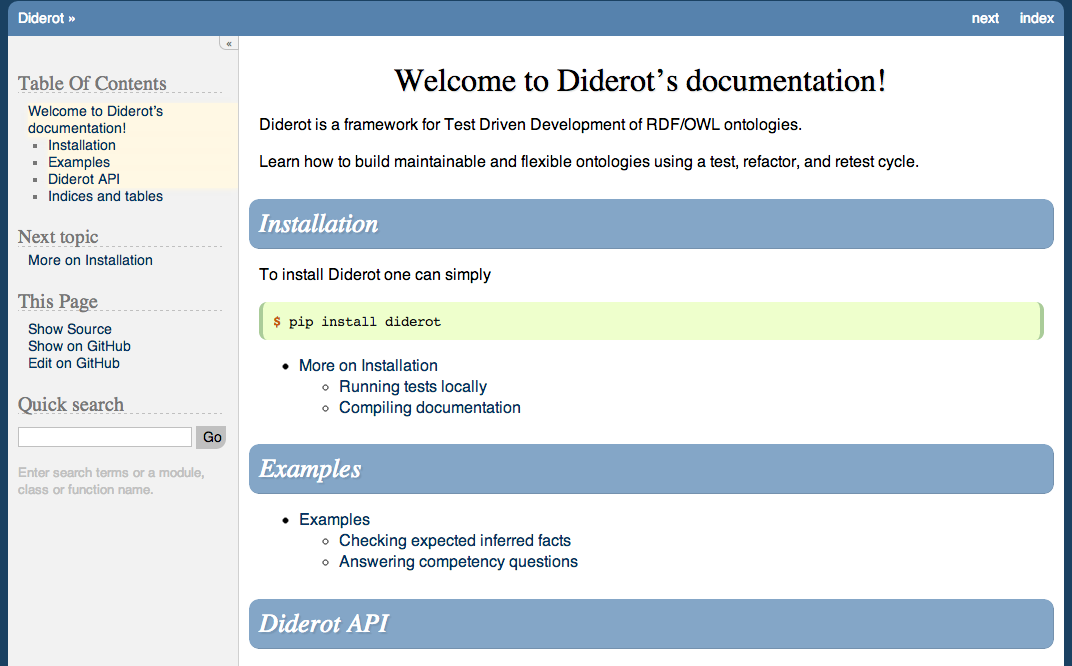
\includegraphics[scale=0.4]{fig/documentation.png}
\end{figure}

\begin{figure}[!hbt]
    \centering
    \label{figDocs2}
    \caption{User manual for checking expected inference use case}
    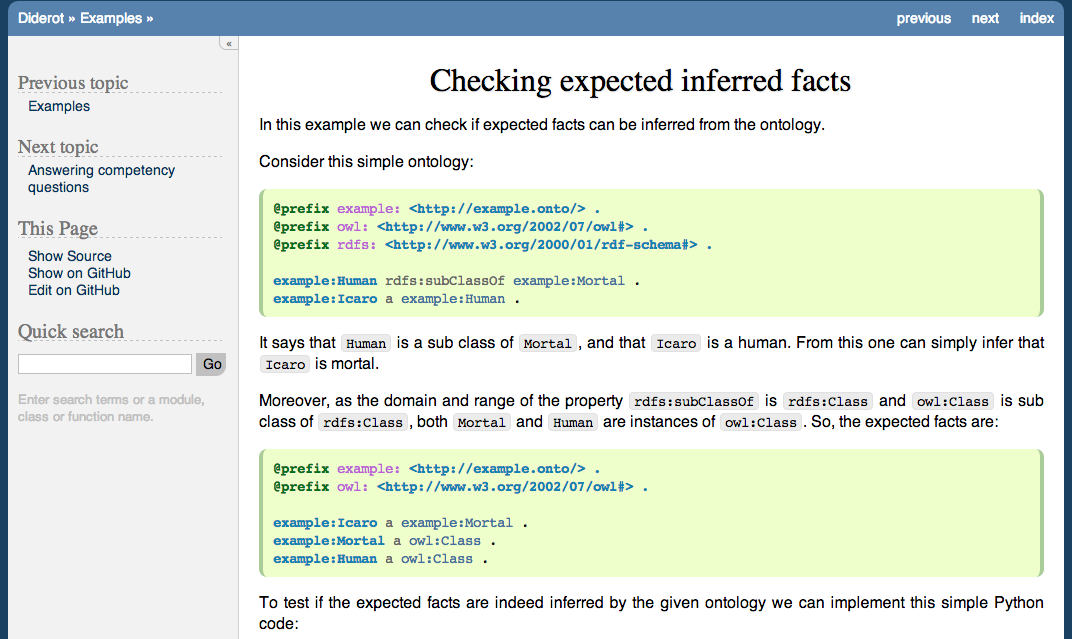
\includegraphics[scale=0.4]{fig/documentation2.png}
\end{figure}

Besides the user documentation, API documentation was created automatically by using docstring code (i.e. comments on method headers) and
the autodoc Sphinx plugin.
This enables programmers to understand how the code works very fast.
It is also useful because API documentation does not need duplication, it is only in code.
An example of our auto-documented API is in Figure \ref{figDocs3}

\begin{figure}[!hbt]
    \centering
    \label{figDocs3}
    \caption{API documentation}
    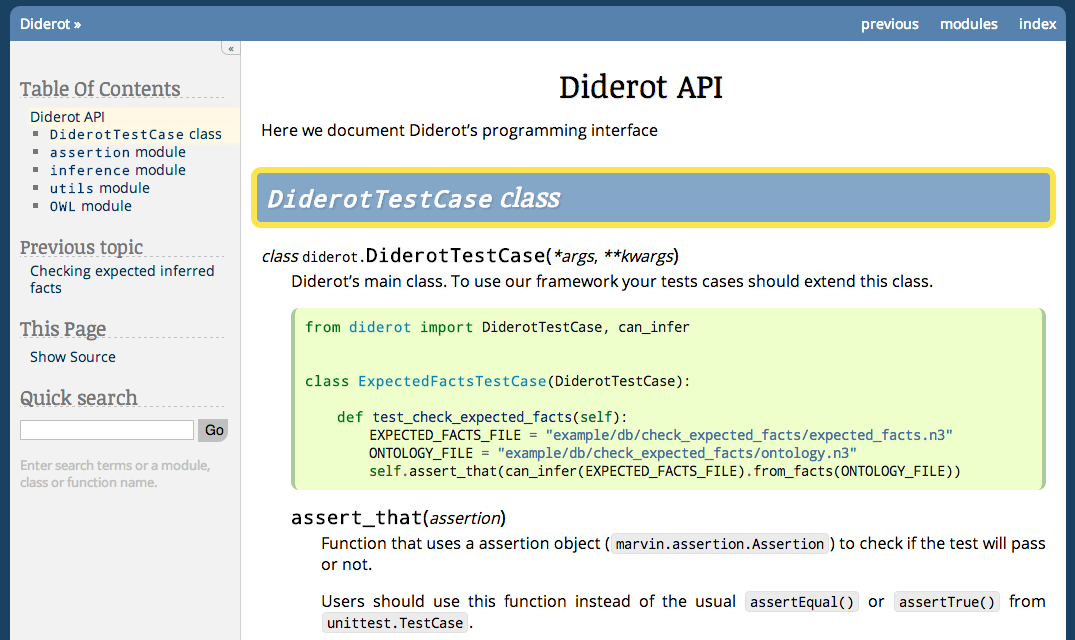
\includegraphics[scale=0.4]{fig/documentation3.png}
\end{figure}


\section{Installation}

To install Diderot, first users need to have Python 2.7 installed \footnote{Other Python versions were not tested. Instructions for installing Python in all platforms can be found in \url{www.python.org/download}}.
Pip tool is also need for installed all the required libraries \footnote{Instruction for installing pip can be found here \url{http://www.pip-installer.org/en/latest/installing.html}}.
It is recommended to use virtualenv tool \footnote{It is recommended to use virtualenv with virtualenvwrapper. Install these tool by using \texttt{pip install virtualenv} and \texttt{pip install virtualenvwrapper}.} to use different environments for Python projects.

After this, simply run \texttt{pip install diderot} and all its dependencies will be installed in the selected virtualenv.

\subsection{Diderot dependencies}

Diderot reuses some libraries to work, namely:

\begin{itemize}
    \item \texttt{rdflib==2.4.2}. Library for parsing RDF files into Python objects, different types of RDF serialization and other facilities for dealing with RDF data.
    \item \texttt{FuXi==1.4.1.production}. Library for OWL inference on Python.
        It is needed to infer facts that can be derived from ontologies.
    \item \texttt{sure==1.2.2}. Library for fluent assertions in Python.

\end{itemize}
\section{Examples}

In this section we describe how to use Diderot, corresponding to the use cases presented in Section \ref{useCases}.

\subsection{Checking Expected Inferences}

In this example we can check if expected facts can be inferred from the ontology.

Consider this simple ontology:

\begin{Verbatim}[commandchars=\\\{\}]
\PYG{k}{@prefix }\PYG{n+nv}{example: }\PYG{n+nn}{\PYGZlt{}http://example.onto/\PYGZgt{} .}
\PYG{k}{@prefix }\PYG{n+nv}{owl: }\PYG{n+nn}{\PYGZlt{}http://www.w3.org/2002/07/owl\PYGZsh{}\PYGZgt{} .}
\PYG{k}{@prefix }\PYG{n+nv}{rdfs: }\PYG{n+nn}{\PYGZlt{}http://www.w3.org/2000/01/rdf\PYGZhy{}schema\PYGZsh{}\PYGZgt{} .}

\PYG{n+nc}{example:Human }\PYG{o}{rdfs:subClassOf }\PYG{n+na}{e}\PYG{n+na}{x}\PYG{n+na}{a}\PYG{n+na}{m}\PYG{n+na}{p}\PYG{n+na}{l}\PYG{n+na}{e}\PYG{n+na}{:}\PYG{n+na}{M}\PYG{n+na}{o}\PYG{n+na}{r}\PYG{n+na}{t}\PYG{n+na}{a}\PYG{n+na}{l }.
\PYG{n+nc}{example:Icaro }\PYG{o}{a }\PYG{n+na}{e}\PYG{n+na}{x}\PYG{n+na}{a}\PYG{n+na}{m}\PYG{n+na}{p}\PYG{n+na}{l}\PYG{n+na}{e}\PYG{n+na}{:}\PYG{n+na}{H}\PYG{n+na}{u}\PYG{n+na}{m}\PYG{n+na}{a}\PYG{n+na}{n }.
\end{Verbatim}

It says that \code{Human} is a sub class of \code{Mortal}, and that \code{Icaro} is a human.
From this one can simply infer that \code{Icaro} is mortal.

Moreover, as the domain and range of the property \code{rdfs:subClassOf} is \code{rdfs:Class} and \code{owl:Class} is sub class of \code{rdfs:Class}, both \code{Mortal} and \code{Human} are instances of \code{owl:Class}. So, the expected facts are:

\begin{Verbatim}[commandchars=\\\{\}]
\PYG{k}{@prefix }\PYG{n+nv}{example: }\PYG{n+nn}{\PYGZlt{}http://example.onto/\PYGZgt{} .}
\PYG{k}{@prefix }\PYG{n+nv}{owl: }\PYG{n+nn}{\PYGZlt{}http://www.w3.org/2002/07/owl\PYGZsh{}\PYGZgt{} .}

\PYG{n+nc}{example:Icaro }\PYG{o}{a }\PYG{n+na}{e}\PYG{n+na}{x}\PYG{n+na}{a}\PYG{n+na}{m}\PYG{n+na}{p}\PYG{n+na}{l}\PYG{n+na}{e}\PYG{n+na}{:}\PYG{n+na}{M}\PYG{n+na}{o}\PYG{n+na}{r}\PYG{n+na}{t}\PYG{n+na}{a}\PYG{n+na}{l }.
\PYG{n+nc}{example:Mortal }\PYG{o}{a }\PYG{n+na}{o}\PYG{n+na}{w}\PYG{n+na}{l}\PYG{n+na}{:}\PYG{n+na}{C}\PYG{n+na}{l}\PYG{n+na}{a}\PYG{n+na}{s}\PYG{n+na}{s }.
\PYG{n+nc}{example:Human }\PYG{o}{a }\PYG{n+na}{o}\PYG{n+na}{w}\PYG{n+na}{l}\PYG{n+na}{:}\PYG{n+na}{C}\PYG{n+na}{l}\PYG{n+na}{a}\PYG{n+na}{s}\PYG{n+na}{s }.
\end{Verbatim}

To test if the expected facts are indeed inferred by the given ontology we can implement this simple Python code:

\begin{Verbatim}[commandchars=\\\{\}]
\PYG{k+kn}{from} \PYG{n+nn}{diderot} \PYG{k+kn}{import} \PYG{n}{DiderotTestCase}\PYG{p}{,} \PYG{n}{can\PYGZus{}infer}


\PYG{k}{class} \PYG{n+nc}{ExpectedFactsTestCase}\PYG{p}{(}\PYG{n}{DiderotTestCase}\PYG{p}{)}\PYG{p}{:}

    \PYG{k}{def} \PYG{n+nf}{test\PYGZus{}check\PYGZus{}expected\PYGZus{}facts}\PYG{p}{(}\PYG{n+nb+bp}{self}\PYG{p}{)}\PYG{p}{:}
        \PYG{n}{EXPECTED\PYGZus{}FACTS\PYGZus{}FILE} \PYG{o}{=} \PYG{l+s}{\PYGZdq{}}\PYG{l+s}{example/db/check\PYGZus{}expected\PYGZus{}facts/expected\PYGZus{}facts.n3}\PYG{l+s}{\PYGZdq{}}
        \PYG{n}{ONTOLOGY\PYGZus{}FILE} \PYG{o}{=} \PYG{l+s}{\PYGZdq{}}\PYG{l+s}{example/db/check\PYGZus{}expected\PYGZus{}facts/ontology.n3}\PYG{l+s}{\PYGZdq{}}
        \PYG{n+nb+bp}{self}\PYG{o}{.}\PYG{n}{assert\PYGZus{}that}\PYG{p}{(}\PYG{n}{can\PYGZus{}infer}\PYG{p}{(}\PYG{n}{EXPECTED\PYGZus{}FACTS\PYGZus{}FILE}\PYG{p}{)}\PYG{o}{.}\PYG{n}{from\PYGZus{}facts}\PYG{p}{(}\PYG{n}{ONTOLOGY\PYGZus{}FILE}\PYG{p}{)}\PYG{p}{)}
\end{Verbatim}

Now consider that we add the triple \code{example:Icaro a example:Student} to the expected facts file.

It is quite obvious that this fact can not be inferred from the ontology.
Then, when running the tests, an \code{AssertionError} will be raised with the expected facts that could not be inferred.

\begin{Verbatim}[commandchars=\\\{\}]
\PYG{g+gp}{\PYGZdl{}} make \PYG{n+nb}{test}
\PYG{g+go}{======================================================================}
\PYG{g+go}{FAIL: test\PYGZus{}some\PYGZus{}expected\PYGZus{}facts\PYGZus{}can\PYGZus{}not\PYGZus{}be\PYGZus{}inferred (test.test\PYGZus{}expected\PYGZus{}facts.ExpectedFactsTestCase)}
\PYG{g+go}{\PYGZhy{}\PYGZhy{}\PYGZhy{}\PYGZhy{}\PYGZhy{}\PYGZhy{}\PYGZhy{}\PYGZhy{}\PYGZhy{}\PYGZhy{}\PYGZhy{}\PYGZhy{}\PYGZhy{}\PYGZhy{}\PYGZhy{}\PYGZhy{}\PYGZhy{}\PYGZhy{}\PYGZhy{}\PYGZhy{}\PYGZhy{}\PYGZhy{}\PYGZhy{}\PYGZhy{}\PYGZhy{}\PYGZhy{}\PYGZhy{}\PYGZhy{}\PYGZhy{}\PYGZhy{}\PYGZhy{}\PYGZhy{}\PYGZhy{}\PYGZhy{}\PYGZhy{}\PYGZhy{}\PYGZhy{}\PYGZhy{}\PYGZhy{}\PYGZhy{}\PYGZhy{}\PYGZhy{}\PYGZhy{}\PYGZhy{}\PYGZhy{}\PYGZhy{}\PYGZhy{}\PYGZhy{}\PYGZhy{}\PYGZhy{}\PYGZhy{}\PYGZhy{}\PYGZhy{}\PYGZhy{}\PYGZhy{}\PYGZhy{}\PYGZhy{}\PYGZhy{}\PYGZhy{}\PYGZhy{}\PYGZhy{}\PYGZhy{}\PYGZhy{}\PYGZhy{}\PYGZhy{}\PYGZhy{}\PYGZhy{}\PYGZhy{}\PYGZhy{}\PYGZhy{}}
\PYG{g+go}{Traceback (most recent call last):}
\PYG{g+go}{  File \PYGZdq{}/path/test\PYGZus{}expected\PYGZus{}facts.py\PYGZdq{}, line 16, in test\PYGZus{}some\PYGZus{}expected\PYGZus{}facts\PYGZus{}can\PYGZus{}not\PYGZus{}be\PYGZus{}inferred}
\PYG{g+go}{    self.assertThat(can\PYGZus{}infer(EXPECTED\PYGZus{}FACTS\PYGZus{}FILE).from\PYGZus{}facts(ONTOLOGY\PYGZus{}FILE))}
\PYG{g+go}{  File \PYGZdq{}/path/diderot/diderot/case.py\PYGZdq{}, line 37, in assertThat}
\PYG{g+go}{    raise AssertionError(ASSERTION\PYGZus{}ERROR\PYGZus{}MESSAGE.format(not\PYGZus{}inferred\PYGZus{}graph.serialize(format=\PYGZdq{}nt\PYGZdq{})))}
\PYG{g+go}{AssertionError: Could not infer some expected facts:}
\PYG{g+go}{  \PYGZlt{}http://example.onto/Icaro\PYGZgt{} \PYGZlt{}http://www.w3.org/1999/02/22\PYGZhy{}rdf\PYGZhy{}syntax\PYGZhy{}ns\PYGZsh{}type\PYGZgt{} }
\PYG{g+go}{     \PYGZlt{}http://example.onto/Student\PYGZgt{}.}
\end{Verbatim}


\subsection{Check Answering to Competency Question}

In this example we can ask to ontologies questions we expect them to answer.

Consider this simple ontology:

\begin{Verbatim}[commandchars=\\\{\}]
\PYG{k}{@prefix }\PYG{n+nv}{example: }\PYG{n+nn}{\PYGZlt{}http://example.onto/\PYGZgt{} .}
\PYG{k}{@prefix }\PYG{n+nv}{owl: }\PYG{n+nn}{\PYGZlt{}http://www.w3.org/2002/07/owl\PYGZsh{}\PYGZgt{} .}
\PYG{k}{@prefix }\PYG{n+nv}{rdfs: }\PYG{n+nn}{\PYGZlt{}http://www.w3.org/2000/01/rdf\PYGZhy{}schema\PYGZsh{}\PYGZgt{} .}
\PYG{k}{@prefix }\PYG{n+nv}{xsd: }\PYG{n+nn}{\PYGZlt{}http://www.w3.org/2001/XMLSchema\PYGZsh{}\PYGZgt{} .}

\PYG{n+nc}{example:Human }\PYG{o}{rdfs:subClassOf }\PYG{n+na}{e}\PYG{n+na}{x}\PYG{n+na}{a}\PYG{n+na}{m}\PYG{n+na}{p}\PYG{n+na}{l}\PYG{n+na}{e}\PYG{n+na}{:}\PYG{n+na}{M}\PYG{n+na}{o}\PYG{n+na}{r}\PYG{n+na}{t}\PYG{n+na}{a}\PYG{n+na}{l }.

\PYG{n+nc}{example:name }\PYG{o}{a           }\PYG{n+na}{o}\PYG{n+na}{w}\PYG{n+na}{l}\PYG{n+na}{:}\PYG{n+na}{D}\PYG{n+na}{a}\PYG{n+na}{t}\PYG{n+na}{a}\PYG{n+na}{t}\PYG{n+na}{y}\PYG{n+na}{p}\PYG{n+na}{e}\PYG{n+na}{P}\PYG{n+na}{r}\PYG{n+na}{o}\PYG{n+na}{p}\PYG{n+na}{e}\PYG{n+na}{r}\PYG{n+na}{t}\PYG{n+na}{y };
             \PYG{o}{rdfs:domain }\PYG{n+na}{e}\PYG{n+na}{x}\PYG{n+na}{a}\PYG{n+na}{m}\PYG{n+na}{p}\PYG{n+na}{l}\PYG{n+na}{e}\PYG{n+na}{:}\PYG{n+na}{H}\PYG{n+na}{u}\PYG{n+na}{m}\PYG{n+na}{a}\PYG{n+na}{n };
             \PYG{o}{rdfs:range  }\PYG{n+na}{x}\PYG{n+na}{s}\PYG{n+na}{d}\PYG{n+na}{:}\PYG{n+na}{s}\PYG{n+na}{t}\PYG{n+na}{r}\PYG{n+na}{i}\PYG{n+na}{n}\PYG{n+na}{g }.

\PYG{n+nc}{example:age }\PYG{o}{a           }\PYG{n+na}{o}\PYG{n+na}{w}\PYG{n+na}{l}\PYG{n+na}{:}\PYG{n+na}{D}\PYG{n+na}{a}\PYG{n+na}{t}\PYG{n+na}{a}\PYG{n+na}{t}\PYG{n+na}{y}\PYG{n+na}{p}\PYG{n+na}{e}\PYG{n+na}{P}\PYG{n+na}{r}\PYG{n+na}{o}\PYG{n+na}{p}\PYG{n+na}{e}\PYG{n+na}{r}\PYG{n+na}{t}\PYG{n+na}{y };
            \PYG{o}{rdfs:domain }\PYG{n+na}{e}\PYG{n+na}{x}\PYG{n+na}{a}\PYG{n+na}{m}\PYG{n+na}{p}\PYG{n+na}{l}\PYG{n+na}{e}\PYG{n+na}{:}\PYG{n+na}{H}\PYG{n+na}{u}\PYG{n+na}{m}\PYG{n+na}{a}\PYG{n+na}{n };
            \PYG{o}{rdfs:range  }\PYG{n+na}{x}\PYG{n+na}{s}\PYG{n+na}{d}\PYG{n+na}{:}\PYG{n+na}{n}\PYG{n+na}{o}\PYG{n+na}{n}\PYG{n+na}{N}\PYG{n+na}{e}\PYG{n+na}{g}\PYG{n+na}{a}\PYG{n+na}{t}\PYG{n+na}{i}\PYG{n+na}{v}\PYG{n+na}{e}\PYG{n+na}{I}\PYG{n+na}{n}\PYG{n+na}{t}\PYG{n+na}{e}\PYG{n+na}{g}\PYG{n+na}{e}\PYG{n+na}{r }.

\PYG{n+nc}{example:Icaro }\PYG{o}{a            }\PYG{n+na}{e}\PYG{n+na}{x}\PYG{n+na}{a}\PYG{n+na}{m}\PYG{n+na}{p}\PYG{n+na}{l}\PYG{n+na}{e}\PYG{n+na}{:}\PYG{n+na}{H}\PYG{n+na}{u}\PYG{n+na}{m}\PYG{n+na}{a}\PYG{n+na}{n };
              \PYG{o}{example:name }\PYG{l+s}{\PYGZdq{}Icaro\PYGZdq{} };
              \PYG{o}{example:age  }\PYG{n+na}{2}\PYG{n+na}{6 }.
\end{Verbatim}

It states that humans (instances of \code{example:Human}) can have name and age.
Moreover, it defines an instance of \code{example:Human}, \code{example:Icaro}, that has a name \code{Icaro} and age of \code{26}.
So, we might want to check if the ontology can answer: is there any humans with the properties names and ages?

In Diderot we can check this by using this simple Python code below.
In lines \code{6-13} we translated the question stated before as a SPARQL query.
Then, in line \code{15}, we call \code{self.assert\_that(can\_answer(QUESTION).from\_ontology(ONTOLOGY\_FILE))} with an ontology file and a question as parameters to check if the ontology can answer the given question.

\begin{Verbatim}[commandchars=\\\{\},numbers=left,firstnumber=1,stepnumber=1]
\PYG{k+kn}{from} \PYG{n+nn}{diderot} \PYG{k+kn}{import} \PYG{n}{DiderotTestCase}\PYG{p}{,} \PYG{n}{can\PYGZus{}answer}

\PYG{k}{class} \PYG{n+nc}{ExpectedFactsTestCase}\PYG{p}{(}\PYG{n}{DiderotTestCase}\PYG{p}{)}\PYG{p}{:}

    \PYG{k}{def} \PYG{n+nf}{test\PYGZus{}check\PYGZus{}can\PYGZus{}answer}\PYG{p}{(}\PYG{n+nb+bp}{self}\PYG{p}{)}\PYG{p}{:}
        \PYG{n}{QUESTION} \PYG{o}{=} \PYG{l+s}{\PYGZdq{}\PYGZdq{}\PYGZdq{}}
\PYG{l+s}{        SELECT ?human ?age ?name}
\PYG{l+s}{        WHERE \PYGZob{}}
\PYG{l+s}{            ?human a                          \PYGZlt{}http://example.onto/Human\PYGZgt{} ;}
\PYG{l+s}{                   \PYGZlt{}http://example.onto/age\PYGZgt{}  26 ;}
\PYG{l+s}{                   \PYGZlt{}http://example.onto/name\PYGZgt{} }\PYG{l+s}{\PYGZdq{}}\PYG{l+s}{Icaro}\PYG{l+s}{\PYGZdq{}}\PYG{l+s}{ .}
\PYG{l+s}{        \PYGZcb{}}
\PYG{l+s}{        }\PYG{l+s}{\PYGZdq{}\PYGZdq{}\PYGZdq{}}
        \PYG{n}{ONTOLOGY\PYGZus{}FILE} \PYG{o}{=} \PYG{l+s}{\PYGZdq{}}\PYG{l+s}{example/db/answering\PYGZus{}competency\PYGZus{}question/ontology.n3}\PYG{l+s}{\PYGZdq{}}
        \PYG{n+nb+bp}{self}\PYG{o}{.}\PYG{n}{assert\PYGZus{}that}\PYG{p}{(}\PYG{n}{can\PYGZus{}answer}\PYG{p}{(}\PYG{n}{QUESTION}\PYG{p}{)}\PYG{o}{.}\PYG{n}{from\PYGZus{}ontology}\PYG{p}{(}\PYG{n}{ONTOLOGY\PYGZus{}FILE}\PYG{p}{)}\PYG{p}{)}
\end{Verbatim}

Only \code{SELECT} and \code{ASK} queries are accepted.
The test will pass if the query result is not empty (for \code{SELECT} queries) or \code{True} (for \code{ASK} queries).

If we ask to the aforementioned ontology if there is any god (that don't exist, at least in the database) the test will fail:

\begin{Verbatim}[commandchars=\\\{\}]
\PYG{g+gp}{\PYGZdl{}} make \PYG{n+nb}{test}
\PYG{g+go}{======================================================================}
\PYG{g+go}{FAIL: test\PYGZus{}is\PYGZus{}there\PYGZus{}a\PYGZus{}god (test.test\PYGZus{}competency\PYGZus{}question\PYGZus{}answering.ExpectedFactsTestCase)}
\PYG{g+go}{\PYGZhy{}\PYGZhy{}\PYGZhy{}\PYGZhy{}\PYGZhy{}\PYGZhy{}\PYGZhy{}\PYGZhy{}\PYGZhy{}\PYGZhy{}\PYGZhy{}\PYGZhy{}\PYGZhy{}\PYGZhy{}\PYGZhy{}\PYGZhy{}\PYGZhy{}\PYGZhy{}\PYGZhy{}\PYGZhy{}\PYGZhy{}\PYGZhy{}\PYGZhy{}\PYGZhy{}\PYGZhy{}\PYGZhy{}\PYGZhy{}\PYGZhy{}\PYGZhy{}\PYGZhy{}\PYGZhy{}\PYGZhy{}\PYGZhy{}\PYGZhy{}\PYGZhy{}\PYGZhy{}\PYGZhy{}\PYGZhy{}\PYGZhy{}\PYGZhy{}\PYGZhy{}\PYGZhy{}\PYGZhy{}\PYGZhy{}\PYGZhy{}\PYGZhy{}\PYGZhy{}\PYGZhy{}\PYGZhy{}\PYGZhy{}\PYGZhy{}\PYGZhy{}\PYGZhy{}\PYGZhy{}\PYGZhy{}\PYGZhy{}\PYGZhy{}\PYGZhy{}\PYGZhy{}\PYGZhy{}\PYGZhy{}\PYGZhy{}\PYGZhy{}\PYGZhy{}\PYGZhy{}\PYGZhy{}\PYGZhy{}\PYGZhy{}\PYGZhy{}\PYGZhy{}}
\PYG{g+go}{Traceback (most recent call last):}
\PYG{g+go}{  File /path/test\PYGZus{}competency\PYGZus{}question\PYGZus{}answering.py\PYGZdq{}, line 51, in test\PYGZus{}is\PYGZus{}there\PYGZus{}a\PYGZus{}god}
\PYG{g+go}{    self.assert\PYGZus{}that(can\PYGZus{}answer(QUESTION).from\PYGZus{}ontology(ONTOLOGY\PYGZus{}FILE))}
\PYG{g+go}{  File /path/case.py\PYGZdq{}, line 30, in assert\PYGZus{}that}
\PYG{g+go}{    raise AssertionError(assertion.assertion\PYGZus{}error\PYGZus{}message)}
\PYG{g+go}{AssertionError: ASK query returned false.}
\PYG{g+go}{  Query:}
\PYG{g+go}{        ASK \PYGZob{}}
\PYG{g+go}{            ?god a \PYGZlt{}http://example.onto/God\PYGZgt{} .}
\PYG{g+go}{        \PYGZcb{}}
\end{Verbatim}

However, in this case we only wanted to check if the ontology \textbf{can} answer the question.
Another useful use case is to check if the ontology can answer the question with a \textbf{specific expected answer}.

This can be done with the Python code below.
The new thing is the argument \code{EXPECTED\_ANSWER} passed to \code{with\_answer()}.
It states expected results for the SPARQL query as a list of tuples of python primitive types (\code{int}, \code{string}, etc) or a \code{RDFlib.URIRef} for URIs.
The tuples should follow the order of the variables in the \code{SELECT} clause in the SPARQL query.
So, the tuple \code{(URIRef("http://example.onto/Icaro"), 26, "Icaro")} match the variables \code{?human, ?age, ?name}, respectively.

\begin{Verbatim}[commandchars=\\\{\},numbers=left,firstnumber=1,stepnumber=1]
\PYG{k+kn}{from} \PYG{n+nn}{diderot} \PYG{k+kn}{import} \PYG{n}{DiderotTestCase}\PYG{p}{,} \PYG{n}{can\PYGZus{}answer}
\PYG{k+kn}{from} \PYG{n+nn}{rdflib} \PYG{k+kn}{import} \PYG{n}{URIRef}

\PYG{k}{class} \PYG{n+nc}{ExpectedFactsTestCase}\PYG{p}{(}\PYG{n}{DiderotTestCase}\PYG{p}{)}\PYG{p}{:}
    \PYG{k}{def} \PYG{n+nf}{test\PYGZus{}check\PYGZus{}can\PYGZus{}answer\PYGZus{}with\PYGZus{}answer}\PYG{p}{(}\PYG{n+nb+bp}{self}\PYG{p}{)}\PYG{p}{:}
        \PYG{n}{QUESTION} \PYG{o}{=} \PYG{l+s}{\PYGZdq{}\PYGZdq{}\PYGZdq{}}
\PYG{l+s}{        SELECT ?human ?age ?name}
\PYG{l+s}{        WHERE \PYGZob{}}
\PYG{l+s}{            ?human a                          \PYGZlt{}http://example.onto/Human\PYGZgt{} ;}
\PYG{l+s}{                   \PYGZlt{}http://example.onto/age\PYGZgt{}  ?age ;}
\PYG{l+s}{                   \PYGZlt{}http://example.onto/name\PYGZgt{} ?name .}
\PYG{l+s}{        \PYGZcb{}}
\PYG{l+s}{        }\PYG{l+s}{\PYGZdq{}\PYGZdq{}\PYGZdq{}}
        \PYG{n}{EXPECTED\PYGZus{}ANSWER} \PYG{o}{=} \PYG{p}{[}\PYG{p}{(}\PYG{n}{URIRef}\PYG{p}{(}\PYG{l+s}{\PYGZdq{}}\PYG{l+s}{http://example.onto/Icaro}\PYG{l+s}{\PYGZdq{}}\PYG{p}{)}\PYG{p}{,} \PYG{l+m+mi}{26}\PYG{p}{,} \PYG{l+s}{\PYGZdq{}}\PYG{l+s}{Icaro}\PYG{l+s}{\PYGZdq{}}\PYG{p}{)}\PYG{p}{]}
        \PYG{n}{ONTOLOGY\PYGZus{}FILE} \PYG{o}{=} \PYG{l+s}{\PYGZdq{}}\PYG{l+s}{example/db/answering\PYGZus{}competency\PYGZus{}question/ontology.n3}\PYG{l+s}{\PYGZdq{}}
        \PYG{n+nb+bp}{self}\PYG{o}{.}\PYG{n}{assert\PYGZus{}that}\PYG{p}{(}\PYG{n}{can\PYGZus{}answer}\PYG{p}{(}\PYG{n}{QUESTION}\PYG{p}{)}\PYG{o}{.}\PYG{n}{from\PYGZus{}ontology}\PYG{p}{(}\PYG{n}{ONTOLOGY\PYGZus{}FILE}\PYG{p}{)}\PYG{o}{.}\PYGZbs{}
                         \PYG{n}{with\PYGZus{}answer}\PYG{p}{(}\PYG{n}{EXPECTED\PYGZus{}ANSWER}\PYG{p}{)}\PYG{p}{)}
\end{Verbatim}

If expected answers and query results are not equal, the test will fail:

\begin{Verbatim}[commandchars=\\\{\}]
\PYG{g+gp}{\PYGZdl{}} make \PYG{n+nb}{test}
\PYG{g+go}{======================================================================}
\PYG{g+go}{FAIL: test\PYGZus{}unexpected\PYGZus{}answer (test.test\PYGZus{}competency\PYGZus{}question\PYGZus{}answering.ExpectedFactsTestCase)}
\PYG{g+go}{\PYGZhy{}\PYGZhy{}\PYGZhy{}\PYGZhy{}\PYGZhy{}\PYGZhy{}\PYGZhy{}\PYGZhy{}\PYGZhy{}\PYGZhy{}\PYGZhy{}\PYGZhy{}\PYGZhy{}\PYGZhy{}\PYGZhy{}\PYGZhy{}\PYGZhy{}\PYGZhy{}\PYGZhy{}\PYGZhy{}\PYGZhy{}\PYGZhy{}\PYGZhy{}\PYGZhy{}\PYGZhy{}\PYGZhy{}\PYGZhy{}\PYGZhy{}\PYGZhy{}\PYGZhy{}\PYGZhy{}\PYGZhy{}\PYGZhy{}\PYGZhy{}\PYGZhy{}\PYGZhy{}\PYGZhy{}\PYGZhy{}\PYGZhy{}\PYGZhy{}\PYGZhy{}\PYGZhy{}\PYGZhy{}\PYGZhy{}\PYGZhy{}\PYGZhy{}\PYGZhy{}\PYGZhy{}\PYGZhy{}\PYGZhy{}\PYGZhy{}\PYGZhy{}\PYGZhy{}\PYGZhy{}\PYGZhy{}\PYGZhy{}\PYGZhy{}\PYGZhy{}\PYGZhy{}\PYGZhy{}\PYGZhy{}\PYGZhy{}\PYGZhy{}\PYGZhy{}\PYGZhy{}\PYGZhy{}\PYGZhy{}\PYGZhy{}\PYGZhy{}\PYGZhy{}}
\PYG{g+go}{Traceback (most recent call last):}
\PYG{g+go}{  File \PYGZdq{}/path/test\PYGZus{}competency\PYGZus{}question\PYGZus{}answering.py\PYGZdq{}, line 75, in test\PYGZus{}unexpected\PYGZus{}answer}
\PYG{g+go}{    with\PYGZus{}answer(EXPECTED\PYGZus{}ANSWER))}
\PYG{g+go}{  File \PYGZdq{}/path/diderot/case.py\PYGZdq{}, line 30, in assert\PYGZus{}that}
\PYG{g+go}{    raise AssertionError(assertion.assertion\PYGZus{}error\PYGZus{}message)}
\PYG{g+go}{AssertionError: Query result is different from expected answer.}
\PYG{g+go}{  given}
\PYG{g+go}{X = [(rdflib.URIRef(\PYGZsq{}http://example.onto/Icaro\PYGZsq{}), \PYGZbs{}}
\PYG{g+go}{      rdflib.Literal(u\PYGZsq{}26\PYGZsq{}, datatype=rdflib.URIRef(\PYGZsq{}http://www.w3.org/2001/XMLSchema\PYGZsh{}integer\PYGZsq{})),\PYGZbs{}}
\PYG{g+go}{      rdflib.Literal(u\PYGZsq{}Icaro\PYGZsq{}))]}
\PYG{g+go}{    and}
\PYG{g+go}{Y = [(rdflib.URIRef(\PYGZsq{}http://example.onto/Icaro\PYGZsq{}), \PYGZbs{}}
\PYG{g+go}{      64, \PYGZbs{}}
\PYG{g+go}{      \PYGZsq{}Icaro Medeiros\PYGZsq{})]}
\PYG{g+go}{X[0][1] is rdflib.Literal(u\PYGZsq{}26\PYGZsq{}, datatype=rdflib.URIRef(\PYGZsq{}http://www.w3.org/2001/XMLSchema\PYGZsh{}integer\PYGZsq{}))}
\PYG{g+go}{  whereas Y[0][1] is 64}
\end{Verbatim}

Note that the query result returns a \code{rdflib.Literal} object, that is transformed to a python primitive type (such as \code{int} or \code{string}) when trying to compare with expected answers if it is not a URI reference.




\chapter{Conclusion}
\label{conclusion}

\section{Future Work}

\begin{appendices}
\chapter{CD Content}

The CD ...

\end{appendices}

\bibliographystyle{plain}
\bibliography{refs}

\end{document}
